% Options for packages loaded elsewhere
\PassOptionsToPackage{unicode}{hyperref}
\PassOptionsToPackage{hyphens}{url}
%
\documentclass[
]{article}
\usepackage{lmodern}
\usepackage{amsmath}
\usepackage{ifxetex,ifluatex}
\ifnum 0\ifxetex 1\fi\ifluatex 1\fi=0 % if pdftex
  \usepackage[T1]{fontenc}
  \usepackage[utf8]{inputenc}
  \usepackage{textcomp} % provide euro and other symbols
  \usepackage{amssymb}
\else % if luatex or xetex
  \usepackage{unicode-math}
  \defaultfontfeatures{Scale=MatchLowercase}
  \defaultfontfeatures[\rmfamily]{Ligatures=TeX,Scale=1}
\fi
% Use upquote if available, for straight quotes in verbatim environments
\IfFileExists{upquote.sty}{\usepackage{upquote}}{}
\IfFileExists{microtype.sty}{% use microtype if available
  \usepackage[]{microtype}
  \UseMicrotypeSet[protrusion]{basicmath} % disable protrusion for tt fonts
}{}
\makeatletter
\@ifundefined{KOMAClassName}{% if non-KOMA class
  \IfFileExists{parskip.sty}{%
    \usepackage{parskip}
  }{% else
    \setlength{\parindent}{0pt}
    \setlength{\parskip}{6pt plus 2pt minus 1pt}}
}{% if KOMA class
  \KOMAoptions{parskip=half}}
\makeatother
\usepackage{xcolor}
\IfFileExists{xurl.sty}{\usepackage{xurl}}{} % add URL line breaks if available
\IfFileExists{bookmark.sty}{\usepackage{bookmark}}{\usepackage{hyperref}}
\hypersetup{
  pdftitle={Group\_07\_Analysis},
  pdfauthor={Group 7},
  hidelinks,
  pdfcreator={LaTeX via pandoc}}
\urlstyle{same} % disable monospaced font for URLs
\usepackage[margin=1in]{geometry}
\usepackage{graphicx}
\makeatletter
\def\maxwidth{\ifdim\Gin@nat@width>\linewidth\linewidth\else\Gin@nat@width\fi}
\def\maxheight{\ifdim\Gin@nat@height>\textheight\textheight\else\Gin@nat@height\fi}
\makeatother
% Scale images if necessary, so that they will not overflow the page
% margins by default, and it is still possible to overwrite the defaults
% using explicit options in \includegraphics[width, height, ...]{}
\setkeys{Gin}{width=\maxwidth,height=\maxheight,keepaspectratio}
% Set default figure placement to htbp
\makeatletter
\def\fps@figure{htbp}
\makeatother
\setlength{\emergencystretch}{3em} % prevent overfull lines
\providecommand{\tightlist}{%
  \setlength{\itemsep}{0pt}\setlength{\parskip}{0pt}}
\setcounter{secnumdepth}{5}
\usepackage{booktabs}
\usepackage{longtable}
\usepackage{array}
\usepackage{multirow}
\usepackage{wrapfig}
\usepackage{float}
\usepackage{colortbl}
\usepackage{pdflscape}
\usepackage{tabu}
\usepackage{threeparttable}
\usepackage{threeparttablex}
\usepackage[normalem]{ulem}
\usepackage{makecell}
\usepackage{xcolor}
\ifluatex
  \usepackage{selnolig}  % disable illegal ligatures
\fi

\title{Group\_07\_Analysis}
\author{Group 7}
\date{}

\begin{document}
\maketitle

\begin{verbatim}
     rating     
 Min.   :0.700  
 1st Qu.:3.700  
 Median :4.700  
 Mean   :5.414  
 3rd Qu.:7.800  
 Max.   :9.200  
\end{verbatim}

\includegraphics{Group_07_Analysis_files/figure-latex/data-1.pdf}

\begin{verbatim}
 Rate      Action   Animation      Comedy Documentary       Drama   Romance
  <=7 37.4% (578)  3.3%  (51) 15.5% (239)  0.7%  (11) 42.0% (650) 1.0% (16)
   >7 14.3% (120) 13.6% (114) 40.8% (343) 14.9% (125)  4.0%  (34) 0.0%  (0)
       Short
  0.1%   (1)
 12.5% (105)
\end{verbatim}

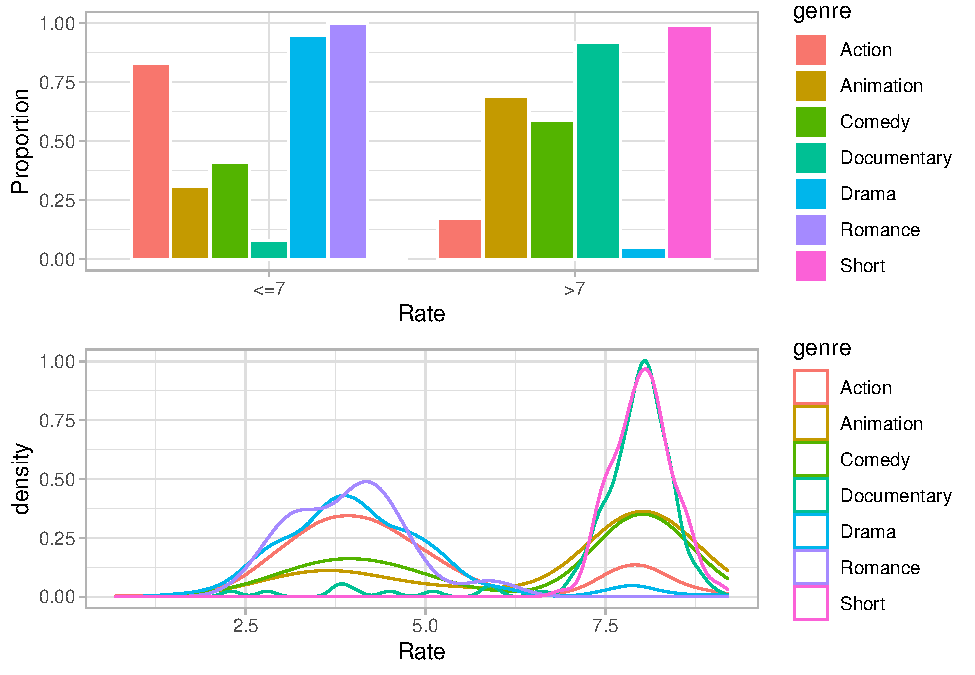
\includegraphics{Group_07_Analysis_files/figure-latex/unnamed-chunk-1-1.pdf}

\begin{verbatim}
.
     Action   Animation      Comedy Documentary       Drama     Romance 
        698         165         582         136         684          16 
      Short 
        106 
\end{verbatim}

\includegraphics{Group_07_Analysis_files/figure-latex/unnamed-chunk-1-2.pdf}

\includegraphics{Group_07_Analysis_files/figure-latex/unnamed-chunk-2-1.pdf}
From this density gragh we can see that Short, Documentary,Comedy and
Animation films are more likely to get rates over 7.5 compared to rates
lower than 7 ( 5 to be exact )

We notice that the majority of films are within one of the 3 most
dominant categories Action , Comedy and Drama . On the opposite
Animation Documentary and Short films have relatively close frequencies
. And Romance films are comparatively very rare among our list of films
( only 16 films where Romantic among all 2387)

\includegraphics{Group_07_Analysis_files/figure-latex/unnamed-chunk-3-1.pdf}

Given the barchart we notice that in our datasel all Romance films have
ratings below 7. This might indicate that Romance is not a strong
explanation a

\includegraphics{Group_07_Analysis_files/figure-latex/unnamed-chunk-4-1.pdf}

\begin{verbatim}
   Min. 1st Qu.  Median    Mean 3rd Qu.    Max.    NA's 
   1.00   72.00   90.00   81.41  100.00  399.00      92 
\end{verbatim}

\begin{verbatim}
[1] 87
\end{verbatim}

\includegraphics{Group_07_Analysis_files/figure-latex/unnamed-chunk-5-1.pdf}
\includegraphics{Group_07_Analysis_files/figure-latex/unnamed-chunk-5-2.pdf}
\includegraphics{Group_07_Analysis_files/figure-latex/unnamed-chunk-5-3.pdf}

\includegraphics{Group_07_Analysis_files/figure-latex/unnamed-chunk-6-1.pdf}

\includegraphics{Group_07_Analysis_files/figure-latex/unnamed-chunk-7-1.pdf}

\includegraphics{Group_07_Analysis_files/figure-latex/unnamed-chunk-8-1.pdf}
\includegraphics{Group_07_Analysis_files/figure-latex/unnamed-chunk-8-2.pdf}
We see in general films' duration are roughly in same range except
Animation and Short films. Both have comperatively smaller lenth

\begin{verbatim}
Call:
glm(formula = Rate ~ genre + length, family = binomial(link = "logit"), 
    data = film)

Deviance Residuals: 
    Min       1Q   Median       3Q      Max  
-2.9520  -0.5677  -0.2469   0.3637   4.1533  

Coefficients:
                   Estimate Std. Error z value Pr(>|z|)    
(Intercept)        1.832605   0.269055   6.811 9.67e-12 ***
genreAnimation    -0.257000   0.299480  -0.858 0.390809    
genreComedy        1.949419   0.143447  13.590  < 2e-16 ***
genreDocumentary   3.989061   0.373338  10.685  < 2e-16 ***
genreDrama        -1.576207   0.222284  -7.091 1.33e-12 ***
genreRomance     -13.669351 348.890679  -0.039 0.968747    
genreShort         3.499947   1.028815   3.402 0.000669 ***
length            -0.038875   0.002934 -13.250  < 2e-16 ***
---
Signif. codes:  0 '***' 0.001 '**' 0.01 '*' 0.05 '.' 0.1 ' ' 1

(Dispersion parameter for binomial family taken to be 1)

    Null deviance: 2982.5  on 2294  degrees of freedom
Residual deviance: 1669.8  on 2287  degrees of freedom
  (92 observations deleted due to missingness)
AIC: 1685.8

Number of Fisher Scoring iterations: 14
\end{verbatim}

\hypertarget{sec:Intro}{%
\section{Introduction}\label{sec:Intro}}

IMDb is a platform that provides information , ratings and reviews on
films, movies and many other streaming content. Our group was given a
dataset taken from this databese, which has records of 2387 films
released from \texttt{r\ min(film\$year)} to 2005 Each film has a unique
identefecation number (id) and some other measurments related to it.
Those are : \textbackslash begin \{itemize\}

\item

\$ Year\_i \$ : the year the film was released at cinemas

\item

\$ Length\_i \$ : duration of film in minutes

\item

\$ Budget\_i\$ : Budget for film production in\$ \$ 10\^{} 5 \$'s

\item

\$ Vote\_i \$ : Number of positive votes

\item

\$ Genre\_i \$ : Genre of film

\item

\$ Rating\_i \$ : IMDb rating from 1 to 10

\textbackslash end \{itemiza\}

\hypertarget{sec:EDA}{%
\section{Exploratory Data Analysis}\label{sec:EDA}}

\begin{table}[!h]

\caption{\label{tab:summary}\label{tab:summary}Summary statistics of variables in the data set.}
\centering
\fontsize{10}{12}\selectfont
\begin{tabular}[t]{lrrrrrrrr}
\toprule
Variable & Mean & SD & Min & Q1 & Median & Q3 & Max & IQR\\
\midrule
Rate & NA & NA & NA & NA & NA & NA & NA & NA\\
year & 1976.872 & 23.739 & 1894.0 & 1958.0 & 1984.0 & 1998.0 & 2005.0 & 14.0\\
length & 81.414 & 37.675 & 1.0 & 72.0 & 90.0 & 100.0 & 399.0 & 10.0\\
budget & 11.948 & 2.968 & 2.1 & 10.0 & 12.0 & 13.9 & 23.7 & 1.9\\
votes & 658.969 & 4370.038 & 5.0 & 12.0 & 32.0 & 118.0 & 103854.0 & 86.0\\
rating & 5.414 & 2.069 & 0.7 & 3.7 & 4.7 & 7.8 & 9.2 & 3.1\\
\bottomrule
\end{tabular}
\end{table}

\begin{verbatim}
     Action   Animation      Comedy Documentary       Drama     Romance 
        698         165         582         136         684          16 
      Short 
        106 
\end{verbatim}

\begin{figure}[H]

{\centering \includegraphics[width=0.68\linewidth]{Group_07_Analysis_files/figure-latex/boxplot -1} 

}

\caption{\label{fig:boxplot}  IMDB rating by genre}\label{fig:boxplot }
\end{figure}

\hypertarget{sec:FDA}{%
\section{Formal Data Analysis}\label{sec:FDA}}

\hypertarget{sec:Conclude}{%
\section{Conclusion and further task}\label{sec:Conclude}}

\end{document}
